\documentclass[11pt]{article}

\usepackage[margin=0.72in]{geometry}
\usepackage{amsmath,amssymb}
\usepackage{array}
\usepackage{booktabs}
\usepackage{caption}
\usepackage{graphicx}
\usepackage{longtable}
\usepackage{tabularx}
\usepackage{xcolor}
\usepackage{hyperref}
\usepackage{microtype}
\usepackage{placeins}

\hypersetup{colorlinks=true,linkcolor=blue!55!black,citecolor=blue!55!black,urlcolor=blue!55!black}
\emergencystretch=2em
\setlength{\tabcolsep}{4.5pt}
\renewcommand{\arraystretch}{1.13}
\newcommand{\pL}{p_{\mathrm L}}
\newcommand{\LKG}{\mathrm{LKG}}
\newcommand{\MM}{\textsc{MM}}
\newcommand{\RTL}{\textsc{RTL}}
\newcolumntype{Y}{>{\raggedright\arraybackslash}X}
\newcolumntype{L}[1]{>{\raggedright\arraybackslash}p{#1}}

\title{Evidence-gated online GKP decoding:\\
parallel multimode qualification and deterministic fail-closed RTL}
\author{}
\date{Phase 6D evidence cutoff: 21 July 2026}

\begin{document}
\maketitle

\begin{abstract}
Online Gottesman--Kitaev--Preskill (GKP) decoding couples two questions that
need not have the same answer: whether an observed-only adaptive decoder
improves logical error rate under drift, and whether a decoder action can be
delivered with deterministic and safe digital semantics.  We separate these
questions into parallel evidence lanes joined by an interface contract rather
than a common performance denominator.  The multimode software lane registers
exact logical-coset maximum-likelihood decoding, static mixture models and
causal adaptive frontends under a common observation and budget contract.  Its
development-only entry test found identical logical error rates for the
strongest retained static-mixture exact-MLD baseline and the proposed causal
risk action, $\pL=0.111979$ over 79,872 rounds, giving a paired relative
improvement and 95\% lower confidence bound of 0\%.  The registered pilot,
formal benchmark and scaling study were therefore not accessed: multimode
frozen-benchmark SOTA is not established.

Independently, the exact single-mode RTL lane integrates the MAP fast path,
event policy, admission logic and versioned A/B parameter banks in one
production top.  It passes 17/17 formal gates and kills 21/21 targeted formal
mutations.  An independent one-million-cycle CXXRTL replay compares the full
148-byte public output vector with zero mismatch, zero undefined action and
zero silent overflow while preserving a six-cycle source-to-action contract
at initiation interval one.  Three open-source placement-and-routing seeds
meet the 27-MHz contract clock; these are whole-harness pre-board estimates,
not physical measurements.  Board latency, jitter, deadline misses and power
remain null, and no FPGA speed advantage is claimed.  CNN and student models
are absent from the primary result and remain replaceable, dropped
approximation modules.  The resulting contribution is a falsifiable
qualification method plus a deterministic, atomic and fail-closed pre-board
implementation, without transferring evidence between the two lanes.
\end{abstract}

\section{Introduction}

GKP codes encode finite-dimensional information in oscillator phase space and
turn small displacement errors into analog modular syndromes
\cite{gkp2001}.  Analog likelihoods can materially improve decoding when the
noise model is known \cite{fukui2018,noh2020}, while multimode lattice geometry
creates a separate algorithmic problem whose solution can range from closest
point decoding \cite{lin2023} to exact logical-coset maximum likelihood and its
$K$-matching approximations \cite{linmld2025,linkmwm2025}.  A deployed
decoder, however, must operate while calibration, correlation and fault
statistics change.  It must also produce actions within a fixed control
deadline and prevent partially validated parameters from reaching the fast
path.

These demands invite an attractive but unsafe narrative: one adaptive model
predicts drift, a neural network improves logical error rate, and an FPGA makes
the resulting decoder fast.  Each clause uses a different task signature.
Logical-error evidence depends on the code, channel, syndrome history,
available actions, comparator and statistical unit.  Hardware evidence depends
on the implemented top, precision, source-to-action boundary, initiation
interval, update transaction and physical transport.  A positive result in one
signature cannot supply a missing denominator in another.  In particular,
short latency in a single-mode lookup path cannot establish multimode decoding
accuracy, and a software LER result cannot prove an RTL safety property.

We therefore formulate an evidence-gated dual-lane system.  The multimode
software lane asks whether observed-only, causal, posterior-aware actions have
prospective headroom over the strongest deployable static decoder.  Its
registered baseline set includes Euclidean and weighted closest-point
decoding, periodic analog-likelihood matching, exact logical-coset MLD
\cite{linmld2025}, $K$-minimum-weight matchings \cite{linkmwm2025}, a
syndrome-estimated static mixture exact MLD,
and causal Window, EWMA, Kalman, SMC and change-point frontends.  The first
question is deliberately cheaper than a full benchmark: if the best causal
action cannot improve the strongest retained baseline on a fresh development
split, more estimator complexity cannot be promoted merely by being trained.

The second lane asks a narrower but constructive hardware question.  Given an
exact single-mode MAP/event design, can one actual RTL top guarantee a
six-cycle, initiation-interval-one action path while accepting parameter
updates atomically and failing closed on invalid data?  This lane uses formal
properties, mutation closure, an independent long-sequence golden model and
whole-harness post-route estimates.  It does not claim that the current RTL
executes the multimode MLD backend, and it reserves all physical-board fields
for a later named-board experiment.  No LER--latency weighted score is defined.

The two contributions are thus parallel.  First, we provide a source-grounded
multimode benchmark and a causal-headroom gate that reaches a negative decision
before pilot or formal data can be inspected.  Second, we provide an exact
single-mode production RTL whose timing and transaction properties are
qualified pre-board.  A shared packet, image and evidence contract explains how
a future multimode compiler could target the same publication mechanism, but
it is not an equivalence proof or a current deployment arrow.  CNN, teacher and
student components have no independent vote: they can approximate an
authorized posterior, likelihood or action only after retention and budget
gates are passed.

This organization changes the paper's claim from ``a CNN--FPGA decoder wins''
to ``a candidate algorithm is allowed to fail its strongest-baseline gate,
while a distinct deterministic hardware contract is proved on the exact top
that exists.''  That separation is the main methodological result.  It also
makes the remaining scientific target unambiguous: a future multimode method
must exceed every eligible deployable baseline with a simultaneous paired
lower confidence bound above the registered 10\% threshold, rather than using
hardware safety or a weaker comparator as evidence of LER superiority.

\section{Related work and task signatures}

\subsection{Static, analog and multimode decoding}

Closest-integer binning is a useful low-cost anchor, but it discards analog
reliability.  Analog matching retains likelihood information
\cite{fukui2018}, and circuit-level surface--GKP studies add repeated noisy
measurements and space--time structure \cite{noh2020}.  Multimode closest-point
decoding instead treats a lattice geometry problem \cite{lin2023}.  These
methods are not interchangeable rows: code family, measurement history and
decoder objective must match before LER values are ranked.  In our target
signature, static-mixture exact logical-coset MLD is the strongest retained
deployable baseline because it marginalizes a frozen syndrome-estimated prior
at the logical-coset level.

\subsection{Adaptation, learned control and physical lifetime}

Syndrome statistics can estimate noise without privileged access to the
latent error \cite{wagner2021}.  Online Window, EWMA, Kalman, particle and
change-point methods differ in delay, memory and their ability to represent
abrupt transitions.  Offline decoder-prior calibration on experimental data
is a valuable but different task \cite{sivak2024}.  Non-Markovian feedback and
learned controllers can optimize a physical protocol when their observation,
action and wall-clock budgets are defined \cite{puviani2025}.  Likewise,
real-time QEC beyond break-even is a physical lifetime claim requiring a
matched device experiment \cite{sivak2023}.  None of those results supplies a
same-task numeric denominator for the present syndrome-only multimode study,
and our per-round simulation does not estimate a physical lifetime.

\subsection{FPGA decoders}

Hardware QEC decoders such as LILLIPUT, Helios and collision-clustering designs
demonstrate important latency and scaling strategies for other code families
\cite{lilliput2022,helios2023,collision2025}.  Raw nanoseconds cannot be ranked
across different syndrome sources, distances, precisions, timing boundaries or
boards.  Our hardware result therefore reports cycles, initiation interval,
formal scope and whole-harness timing closure.  It makes no claim to be faster
than an existing FPGA decoder.

\section{Methods}

\subsection{Two-lane evidence contract}

An evidence lane is a tuple
\begin{equation}
  \mathcal T=(\mathcal C,\mathcal N,\mathcal O,\mathcal A,
  \mathcal D,\mathcal P,\mathcal B,\mathcal M,\mathcal S),
\end{equation}
where $\mathcal C$ is the code family, $\mathcal N$ the channel, $\mathcal O$
the online observations, $\mathcal A$ the action space, $\mathcal D$ the
decoder backend, $\mathcal P$ the precision, $\mathcal B$ the compute budget,
$\mathcal M$ the metric namespace and $\mathcal S$ the statistical unit.  A
claim may move between methods only when these fields match or when an explicit
adapter and its error are qualified.  The software and RTL lanes share
versioned packet/image interfaces and fail-closed publication semantics; they
do not share $\mathcal C$, $\mathcal D$, $\mathcal M$ or $\mathcal S$.

Three transfers are forbidden throughout this work.  An RTL property cannot
rescue a failed multimode LER gate.  A multimode simulation cannot validate an
RTL timing or safety property.  A learned approximation cannot alter either
primary verdict unless its own matched retention, precision and resource gates
are passed.  Consequently, no LER--latency weighted score is defined.

\subsection{Multimode software qualification lane}

The deployable software record contains quantized syndromes and health fields
available up to the current decision.  Latent drift state, scenario identity,
future samples and logical labels are isolated in an evaluator record.  Prefix,
future-suffix and truth-mutation tests check that the deployable path is
observed-only.  The exact logical-coset backend computes
\begin{equation}
  \widehat L_t=\arg\max_L
  \int p(L,s_t\mid\theta)\,p(\theta\mid s_{<t})\,d\theta,
\end{equation}
with a point prior recovering plug-in exact MLD.  A static mixture freezes
$p(\theta)$ from the allowed pre-formal data and is therefore deployable.

The registered development entry test uses 12 seeds, 13 drift families and
512 rounds per family, or 79,872 paired rounds per method.  All methods see the
same trace.  Baseline selection, causal ceiling and action-value decomposition
are computed before any pilot or formal access.  Continuation requires at
least 15\% point headroom and a 12\% paired 95\% lower confidence bound over the
strongest retained development baseline.  Failure stops implementation,
pilot, formal and scaling tasks.  The later frozen-benchmark promotion rule is
stricter: the simultaneous paired lower bound must exceed 10\% against every
eligible deployable baseline, with a positive absolute lower bound and
consistent $d=3,5$ behavior at registered noise points.

We also preserve an earlier opened task-local multimode experiment.  It uses a
different denominator and was inspected before the Phase 6D split; hence its
LER, tail and host-runtime values are descriptive context, not a ranking result
and not evidence for the registered promotion gate.

\subsection{Exact single-mode RTL lane}

The production top instantiates the parameter-bank manager, commit admission,
five-stage MAP core and one-stage event/action policy exactly once.  There is
no raw configuration or trust bypass into the core.  The source-to-action
contract is
\begin{equation}
  t_{\mathrm{action}}-t_{\mathrm{source}}=6\ \text{cycles},
  \qquad \mathrm{II}=1.
\end{equation}
The contract ends at the registered RTL output and excludes physical transport,
CDC, ADC/DAC and control electronics.

Each update stages a complete image in the inactive bank.  Admission checks
image completeness, CRC, version, expected active bank and trust state.  A
compare-and-swap commit occurs only at a safe boundary; the retired bank is
protected for the six-cycle pipeline drain.  Integrity, age, leakage,
posterior-sum or version faults select a defined fallback and can republish the
last-known-good image.  Image generation and activation epochs are distinct,
so a trusted older image may be restored without pretending that its payload
was regenerated.

Formal qualification covers all-state management/admission guards, transition
refinement, bounded reachability, the actual core's fail-closed output and
three-step atomic commit behavior.  Cover traces exercise activation, LKG
recovery, cancellation, drain rejection, near-wrap rejection, host conflict and
policy priority.  Targeted semantic mutations remove or corrupt one protection
at a time; a property suite is accepted only if every registered mutation is
killed.

The independent long-sequence model reimplements admission, management, core
and policy behavior without importing the RTL implementation.  It compares a
148-byte public vector cycle by cycle over ten 100,000-cycle families.  The
trace includes full-image transactions, host/policy commit races, rejected
updates, integrity faults, leakage, recovery and compound transport events.
Post-route qualification uses the same whole-harness observability top and
three fixed seeds.  Frequency and resources are estimates from the open-source
flow; no vendor timing signoff or physical-board measurement is inferred.

\subsection{Replaceable CNN/student extension}

A learned module is permitted only as an approximation to an authorized
posterior, log-likelihood ratio, logical-coset probability or action.  It must
use the same train/calibration/pilot/formal split and online information as its
teacher, and must report calibration, action agreement, LER retention,
worst-family retention, runtime, memory and quantization error under a matched
budget.  Phase 6D did not authorize the teacher because the multimode entry
test stopped before implementation.  CNN/student training, quantization and
formal retention were therefore not run, and legacy CNN evidence cannot reopen
either primary lane.

\subsection{Evidence states and reproducibility}

We use distinct states for measured, estimated, reproduced, contextual,
negative, dropped, blocked and not-applicable values.  Null is not zero.  Every
primary statement is bound to a report, raw data or trace, configuration,
implementation, source locator and SHA-256 hash.  Negative decisions retain
their denominator and unavailable downstream outputs.  The machine contract
rejects mutations that delete the strongest baseline, fill a board-null field,
promote learning, merge lane metrics or reuse a historical figure as current
evidence.

\section{Results}

\subsection{The multimode causal-headroom gate is negative}

The strongest development baseline was static-mixture exact MLD.  It and the
best causal risk action each made 8,944 logical errors in 79,872 paired rounds,
giving
\begin{equation}
  \pL^{\mathrm{static\ mixture\ MLD}}
  =\pL^{\mathrm{causal\ risk}}=0.1119791667.
\end{equation}
The paired relative improvement was 0\%, with a 95\% lower confidence bound of
0\%.  Both the 15\% point and 12\% lower-bound entry thresholds failed.  The
verdict was therefore \texttt{NO\_GO\_MULTIMODE\_CAUSAL\_HEADROOM}; no proposed
posterior-predictive implementation was selected, and pilot, formal and
distance/noise scaling were not accessed.

The decomposition explains why additional estimator capacity was not a
promising rescue.  Relative to intermediate variants, the observed-only
estimator, metric, coset, marginalization and action components contributed
$-0.001277$, $-0.033654$, $-0.014636$, $-0.000013$ and $+0.055551$ absolute LER,
respectively.  The trusted action intervened 9,884 times and removed 4,437
errors relative to the unprotected action variant, but only returned the
system to the static-mixture exact-MLD result.  The action policy repaired
errors created upstream; it did not create net headroom over the strongest
static decoder.

\begin{figure}[htbp]
  \centering
  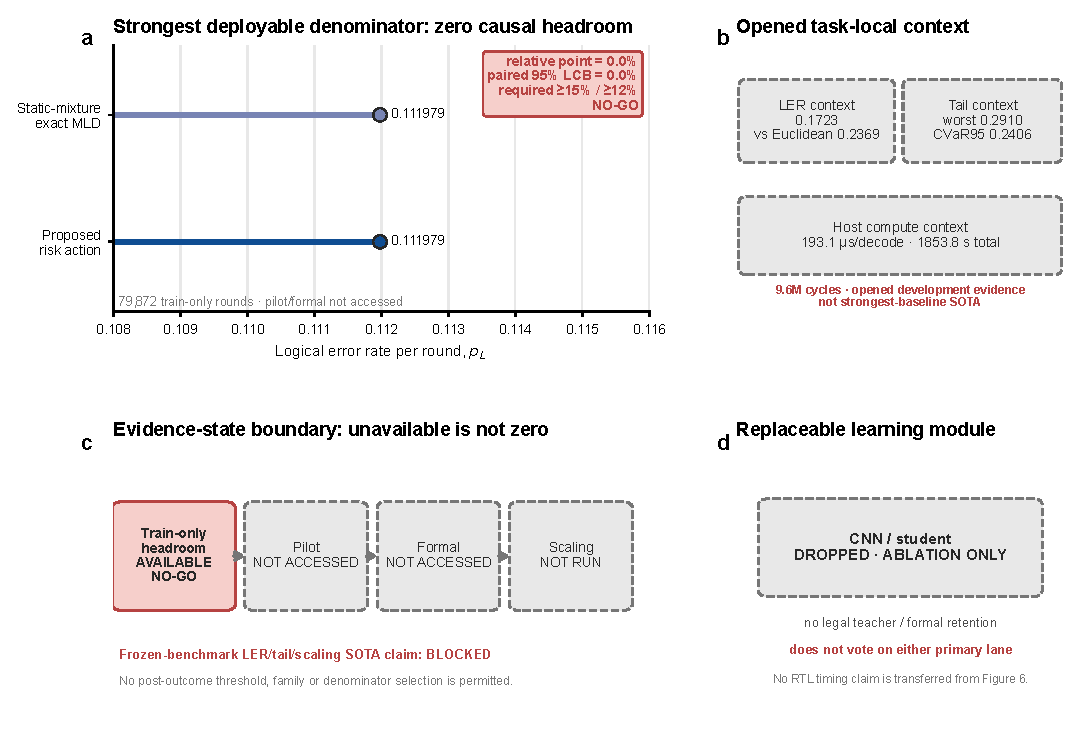
\includegraphics[width=\textwidth]{../figures/t7_1_5_phase6d_delta/figure5_multimode_software_delta.pdf}
  \caption{Multimode software evidence.  (a) The strongest-baseline entry
  comparison has zero point and lower-bound headroom.  (b) An opened $d=3$
  task-local study is retained only as LER, tail and host-compute context
  because it does not use the strongest denominator.  (c) Pilot, formal and
  scaling evidence remain not run after the entry stop.  (d) CNN/student is a
  dropped ablation state.  No RTL result is used to alter this verdict.}
  \label{fig:mm-delta}
\end{figure}

\subsection{Opened multimode results remain contextual}

The earlier opened $d=3$ study processed 9.6 million physical cycles across 32
seed clusters with 20,000 bootstrap resamples.  The candidate had
$\pL=0.17226094$ versus $0.23692938$ for static Euclidean decoding, an absolute
difference of $0.06466844$ with interval $[0.06441281,0.06492636]$.  Its
non-overlapping 512-cycle worst-window LER was $0.291015625$, CVaR95 was
$0.24062667$, and measured host runtime was 1853.802 s.  These values show that
the simulator and tail accounting are operational.  They do not establish
SOTA because static Euclidean decoding is weaker than the subsequently retained
static-mixture exact MLD and the data belong to an opened, task-local context.

\subsection{The exact single-mode RTL passes deterministic and safety gates}

All 17 registered formal gates passed, and all 21 targeted formal mutations
were killed.  The proof scope includes inductive safety invariants and
transition refinement for the converged top, bounded reachability, and direct
properties on the actual MAP core.  It does not include unbounded liveness,
physical CDC/metastability or a multimode decoder.

The independent CXXRTL qualification processed 1,000,000 cycles.  Of these,
998,462 had valid inputs and outputs.  All 998,435 adjacent valid input pairs
produced adjacent outputs, confirming II=1.  The observed source-to-action
latency was exactly six cycles and MAP latency exactly five cycles.  Full-vector
comparison found zero mismatch, zero latency violation, zero undefined action,
zero CRC error and zero silent version wrap or arithmetic overflow.  The run
included 4 completed bank commits, 28 management rejects, 471 fault-to-clean
recoveries and 882 route-to-open recoveries rather than a nominal-only trace.

\begin{figure}[htbp]
  \centering
  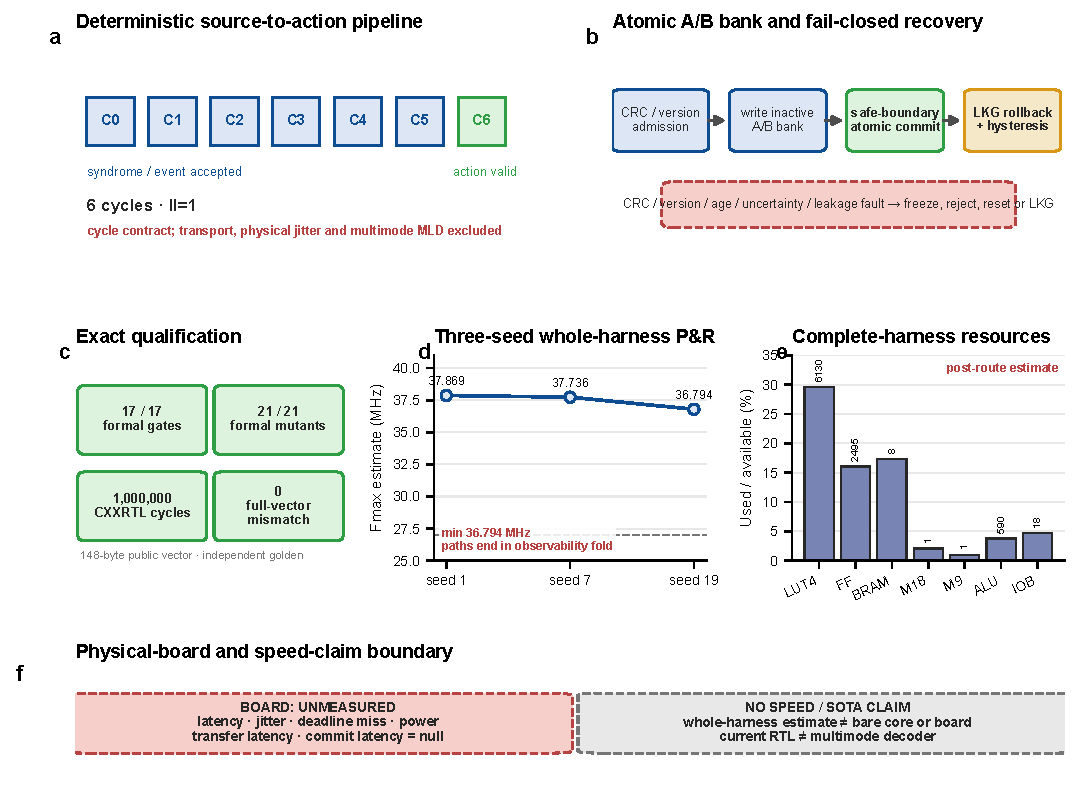
\includegraphics[width=\textwidth]{../figures/t7_1_5_phase6d_delta/figure6_single_mode_rtl_delta.pdf}
  \caption{Exact single-mode pre-board RTL evidence.  (a) The source-to-action
  contract is six cycles at II=1.  (b) CRC/version admission, inactive-bank
  staging, safe-boundary commit and LKG recovery implement atomic fail-closed
  publication.  (c) Formal and one-million-cycle CXXRTL qualification pass.
  (d,e) Three post-route seeds meet 27 MHz for the whole observability harness;
  resources and frequency are estimates.  (f) Board latency, jitter, deadline
  misses, power and physical transaction latency remain null.  The current RTL
  does not execute the multimode decoder.}
  \label{fig:rtl-delta}
\end{figure}

All three placement-and-routing seeds met the 27-MHz contract clock.  Estimated
Fmax ranged from 36.794 to 37.869 MHz with a median of 37.736 MHz.  Median
whole-harness resources were 6,118 LUT4, 2,495 DFF, 8 BSRAM, one 18x18
multiplier and one 9x9 multiplier.  Critical paths terminated in the
observability fold, so the frequency is not relabelled as a bare-core result.
The six-cycle clock model corresponds to 222.222 ns at 27 MHz and 163.068 ns at
minimum estimated Fmax, but neither number includes transport or physical
jitter and neither is a board measurement.

\subsection{The combined verdict is RTL-only}

The two Boolean lane decisions are multimode=false and RTL=true.  The resulting
publication verdict is \texttt{GO\_RTL\_ONLY}: the exact single-mode
deterministic/atomic/fail-closed pre-board contribution is open, while
multimode SOTA, learning promotion, board measurement and FPGA speed ranking
remain closed.  No scalar combines LER with cycles or resources.  The positive
RTL lane neither compensates for nor weakens the mandatory multimode negative.

\section{Discussion}

The principal lesson is that algorithmic adaptivity and safe deterministic
execution are separable scientific claims.  The multimode result is
informative precisely because it prevents a large engineering effort after a
strong static model erased the apparent causal gain.  Against static
Euclidean decoding the opened study looked favorable; against static-mixture
exact MLD the registered causal ceiling had zero headroom.  This is consistent
with a regime in which past syndromes identify enough of a stationary mixture
for a frozen marginal decoder, while real-time state estimates are too noisy or
too delayed to change the logical action profitably.

The decomposition also clarifies what must change before a renewed multimode
claim is credible.  A future proposal needs new causal information or a new
action space, not simply a larger predictor.  Candidate directions include
sensor-side calibration variables that are genuinely available online,
longer-horizon posterior prediction validated prequentially, or physical
control actions whose counterfactual value exceeds the static decoder.  Each
would require a fresh immutable split and the same strongest baseline set.  It
would not be permissible to tune thresholds separately on calibration and
telegraph families after seeing the formal result.

The RTL contribution solves a different failure mode.  An estimator can be
statistically useful and still publish a torn, stale or untrusted image, miss a
deadline, or return an undefined action.  The converged top makes the safety
authority explicit: full-image staging, versioned compare-and-swap, pipeline
drain and LKG recovery are part of the decoder interface.  Formal mutation and
long-sequence fault traffic provide stronger pre-board evidence than a
nominal demo.  Nevertheless, fail closed is a digital invariant, not a claim
that the fallback action minimizes LER or that the physical system is safe.

The contract bridge is consequently architectural rather than empirical.  A
future multimode compiler may target versioned images and the same transaction
protocol, but it must first prove quantization and action equivalence, meet the
six-cycle/II=1 or a newly registered timing contract, and repeat formal,
mutation, long-sequence and post-route qualification on the new actual top.
Until then the current hardware remains exact single mode.  This boundary is
what prevents two individually valid results from becoming one invalid global
claim.

Learning remains optional by construction.  A CNN or student could reduce
posterior cost or approximate exact MLD if it preserved calibration, actions,
LER and worst-family behavior under a matched resource budget.  Phase 6D
contains no authorized teacher or formal retention result, so making learning
central would add a third unsupported claim rather than strengthen the two
lanes.  The appropriate current use is an explicit dropped ablation and a
future replaceable module.

\section{Limitations}

The multimode experiment is simulation-based.  The registered development
headroom result covers the frozen $d=3$ task signature but did not continue to
the $d=3,5$ pilot/formal/scaling matrix.  It does not establish a universal
impossibility of adaptive GKP decoding.  Some source-backed comparators were
registered but remained ineligible or unexecuted after the stop, including
periodic analog-likelihood MWPM, $K$-MWM, source-transcribed noisy-auxiliary
decoding, SMC, BOCPD and IMM.  The correct conclusion is a Phase 6D v1 no-go,
not that static MLD always dominates adaptation.

The hardware scope is a two-state, exact single-mode digital top.  Formal and
CXXRTL evidence exclude physical transport, pin constraints, CDC,
metastability, analog acquisition, control electronics and the quantum device.
Placement and routing use an open-source flow rather than vendor signoff.  The
reported 27-MHz clock and Fmax values are pre-board estimates.  Physical-board
latency, jitter, deadline misses, power, transfer latency and commit latency are
unmeasured and stored as null.  We therefore claim neither measured speed nor
an advantage over existing FPGA QEC decoders.

Finally, per-round simulated LER cannot be compared with the logical lifetime
or break-even values of a cavity experiment or a non-Markovian feedback
controller.  The present work contains no calibrated cavity--transmon digital
twin, real GKP record, closed-loop quantum-device action, measured logical
lifetime or physical break-even result.  Those claims require a separate
protocol-matched experiment.

\section{Reproducibility and evidence availability}

Figure~\ref{fig:mm-delta} and Figure~\ref{fig:rtl-delta} are generated from a
94-row lossless Source Data contract that binds 13 figure elements, 10 final
claims, 11 read-only historical snapshots and 58 live artifacts.  The figure
contract passes 22/22 gates and 22/22 semantic mutations.  The multimode
headroom report stores all 79,872 paired decisions and the component
decomposition.  The RTL package stores formal commands and outputs, mutation
results, the 202-MB long trace, the independent golden output, all 148 public
bytes per cycle, synthesis/netlist logs and every placement-and-routing seed.

The canonical current manuscript is this file.  The earlier 51-page
contract-centric note and T7.1.1--T7.2.5 contracts remain immutable historical
snapshots; their V4 or Phase 6C claims do not override the Phase 6D final gate.
The Supplement below provides the delta needed to interpret those snapshots.

\section{Conclusion}

We present two parallel results without combining their denominators.  The
multimode software lane contributes a strong-baseline registry and a
prospective causal-headroom gate; its v1 candidate has 0\% improvement and 0\%
paired lower-bound headroom over static-mixture exact MLD, so frozen-benchmark
LER SOTA is not established.  The exact single-mode hardware lane contributes
a six-cycle, II=1 converged RTL that passes formal mutation closure,
one-million-cycle independent full-vector equivalence and three-seed
whole-harness timing closure, with atomic A/B publication and fail-closed LKG
recovery.

The evidence boundary is part of the result.  The current RTL does not execute
the multimode MLD, learning is dropped to an optional approximation, and all
physical-board fields remain null.  Thus this work establishes deterministic,
atomic and fail-closed pre-board execution for the exact single-mode design,
not multimode SOTA, physical lifetime gain or fastest-FPGA status.  The next
positive algorithmic paper must first create and prospectively demonstrate
causal action-value headroom against the same strongest deployable baseline.

\clearpage
\appendix

\section{Supplementary delta: terminology and evidence states}

\begin{longtable}{@{}L{0.24\textwidth} L{0.25\textwidth} L{0.43\textwidth}@{}}
\caption{Canonical terminology for the Phase 6D manuscript.}\label{tab:terms}\\
\toprule
Term & Meaning & Excluded interpretation \\
\midrule
\endfirsthead
\toprule
Term & Meaning & Excluded interpretation \\
\midrule
\endhead
Multimode software lane & Registered simulation task for algorithmic LER qualification & Not implemented in current RTL \\
Exact single-mode RTL lane & Two-state production top qualified for cycles and digital safety & Not a multimode or physical-device decoder \\
Static-mixture exact MLD & Frozen syndrome-estimated prior marginalized at logical-coset level & Not a truth-privileged oracle \\
Opened task-local context & Inspected result with a weaker/different denominator & Not frozen-benchmark evidence \\
Frozen-benchmark SOTA & Simultaneous $>10\%$ paired LCB against every eligible baseline & Not reached in Phase 6D \\
Six-cycle, II=1 & Registered RTL source-to-action cycle contract & Not measured nanoseconds including transport \\
Whole-harness post-route estimate & Timing/resource result for the observability top & Not bare-core, vendor-signoff or board measurement \\
Board-null & Measurement was not performed and the value is null & Not zero latency, jitter, deadline misses or power \\
CNN/student dropped ablation & Optional approximation without an authorized teacher/formal retention & Not a primary contribution \\
\bottomrule
\end{longtable}

\section{Supplementary delta: baseline eligibility}

\begin{longtable}{@{}L{0.24\textwidth} L{0.22\textwidth} L{0.18\textwidth} L{0.28\textwidth}@{}}
\caption{Multimode baseline registry and Phase 6D disposition.}\label{tab:baselines}\\
\toprule
Method & Role & Phase 6D state & Ranking boundary \\
\midrule
\endfirsthead
\toprule
Method & Role & Phase 6D state & Ranking boundary \\
\midrule
\endhead
Closest integer & Weak sanity anchor & Registered & Never strongest \\
Euclidean CPD/MWPM & Official geometric baseline & Context & Same-task only \\
Weighted CPD & Static/adaptive metric adapter & Registered & Adapter, not source-exact \\
Periodic analog MWPM & Folded-likelihood comparator & Dropped after stop & Cannot be replaced by Euclidean weights \\
Exact logical-coset MLD & Strong backend & Registered & Explicit-coset checks required \\
$K$-MWM & Accuracy--cost approximation & Dropped after stop & Full $K$--LER--cost curve required \\
Static-mixture exact MLD & Strongest frozen static candidate & Executed in entry test & Primary development denominator \\
Delayed Window & Causal adaptive frontend & Registered & No future-window samples \\
EWMA/Kalman & Causal adaptive frontends & Registered & Common calibration and cadence \\
SMC-EAP & Adapted posterior baseline & Dropped after stop & Must be labelled adapted \\
BOCPD/IMM & Abrupt-drift baselines & Dropped after stop & Hazard/states frozen on calibration \\
True-$\theta$ exact MLD & Evaluation upper bound & Not ranked & Truth privilege prohibited online \\
\bottomrule
\end{longtable}

Roy--Pousset--Royer noisy-auxiliary decoding, repeated circuit-level
surface--GKP decoding, Puviani NMF, AQEC, experimental prior calibration and
existing FPGA decoders remain separate protocol lanes.  They may provide
mechanistic context but cannot enter a numeric global leaderboard without an
exact observation/action/environment/budget match.

\section{Supplementary delta: complete claim boundary}

\begin{longtable}{@{}L{0.22\textwidth} L{0.16\textwidth} L{0.23\textwidth} L{0.31\textwidth}@{}}
\caption{Final claims consumed by the manuscript.}\label{tab:claims}\\
\toprule
Claim & State & Current evidence & Required boundary \\
\midrule
\endfirsthead
\toprule
Claim & State & Current evidence & Required boundary \\
\midrule
\endhead
Opened multimode gain & Context only & 9.6M-cycle task-local study & Not strongest denominator \\
Multimode causal headroom & Mandatory negative & 0\% point and LCB vs static-mixture exact MLD & Pilot/formal unaccessed \\
Frozen-benchmark SOTA & Blocked & No formal result or simultaneous $>10\%$ LCB & Must remain unclaimed \\
Deterministic RTL & Restricted positive & Six cycles, II=1, 1M-cycle full-vector replay & Exact single-mode pre-board only \\
Atomic/fail-closed RTL & Restricted positive & 17/17 formal gates; 21/21 mutants & Digital/two-state scope \\
Post-route estimate & Restricted positive & Three seeds; minimum Fmax 36.794 MHz & Whole harness; no vendor signoff \\
Board measurement & Blocked & All physical fields null & No measured timing/power \\
FPGA speed advantage & Prohibited positive & No same-task board comparator & No fastest/SOTA wording \\
CNN/student & Dropped ablation & No teacher, checkpoint or retention result & No vote in either lane \\
Dual-lane relation & Mandatory boundary & Global weighted score is null & Contract bridge only \\
\bottomrule
\end{longtable}

\section{Supplementary delta: revocation and negative-result audit}

The manuscript contract is revoked if any of the following occurs: the
static-mixture exact-MLD row is deleted; the 0\% headroom is omitted; the
opened result is called formal or SOTA; pilot/scaling nulls are filled with
zeros; the current RTL is said to run multimode MLD; a post-route clock model
is described as board measured; a physical deadline or power value is
invented; CNN/student is made primary; a common LER--latency score is added; or
one lane is allowed to satisfy the other lane's gate.

The negative result has complete denominators rather than an absence-only
assertion: 12 seeds, 13 families, 512 rounds, 79,872 total paired rounds, a
named strongest baseline, exact error counts, paired point and lower-bound
effects, registered continuation thresholds and an explicit list of unaccessed
downstream stages.  The RTL positive result likewise includes non-nominal
traffic, rejected transactions, recovery events, every public output byte,
three place-and-route seeds and a stated physical exclusion surface.

\section{Supplementary delta: historical snapshot policy}

T7.1.1--T7.1.4 and T7.2.1--T7.2.5 are read-only Phase 6C snapshots.  They
remain useful for provenance, earlier V4 negative results, method definitions
and external-comparison source locators.  Their restricted manuscript verdict
cannot override the later Phase 6D truth table.  Figures 5 and 6 use new output
paths and do not overwrite Figures 1--4 or Supplementary Figures S1--S5.

For release, every historical snapshot is identified by path and SHA-256 hash,
and the current manuscript contract verifies all live Phase 6D parents.  A
source, configuration, report or code hash drift invalidates the generated
delta until the corresponding experiment and claim gate are rerun.

\bibliographystyle{unsrt}
\bibliography{CNN_FPGA_GKP_submission_refs,Phase6D_Dual_Lane_GKP_refs}

\end{document}
